\documentclass{standalone}
\usepackage{tikz}
\usetikzlibrary{patterns, positioning}

\begin{document}
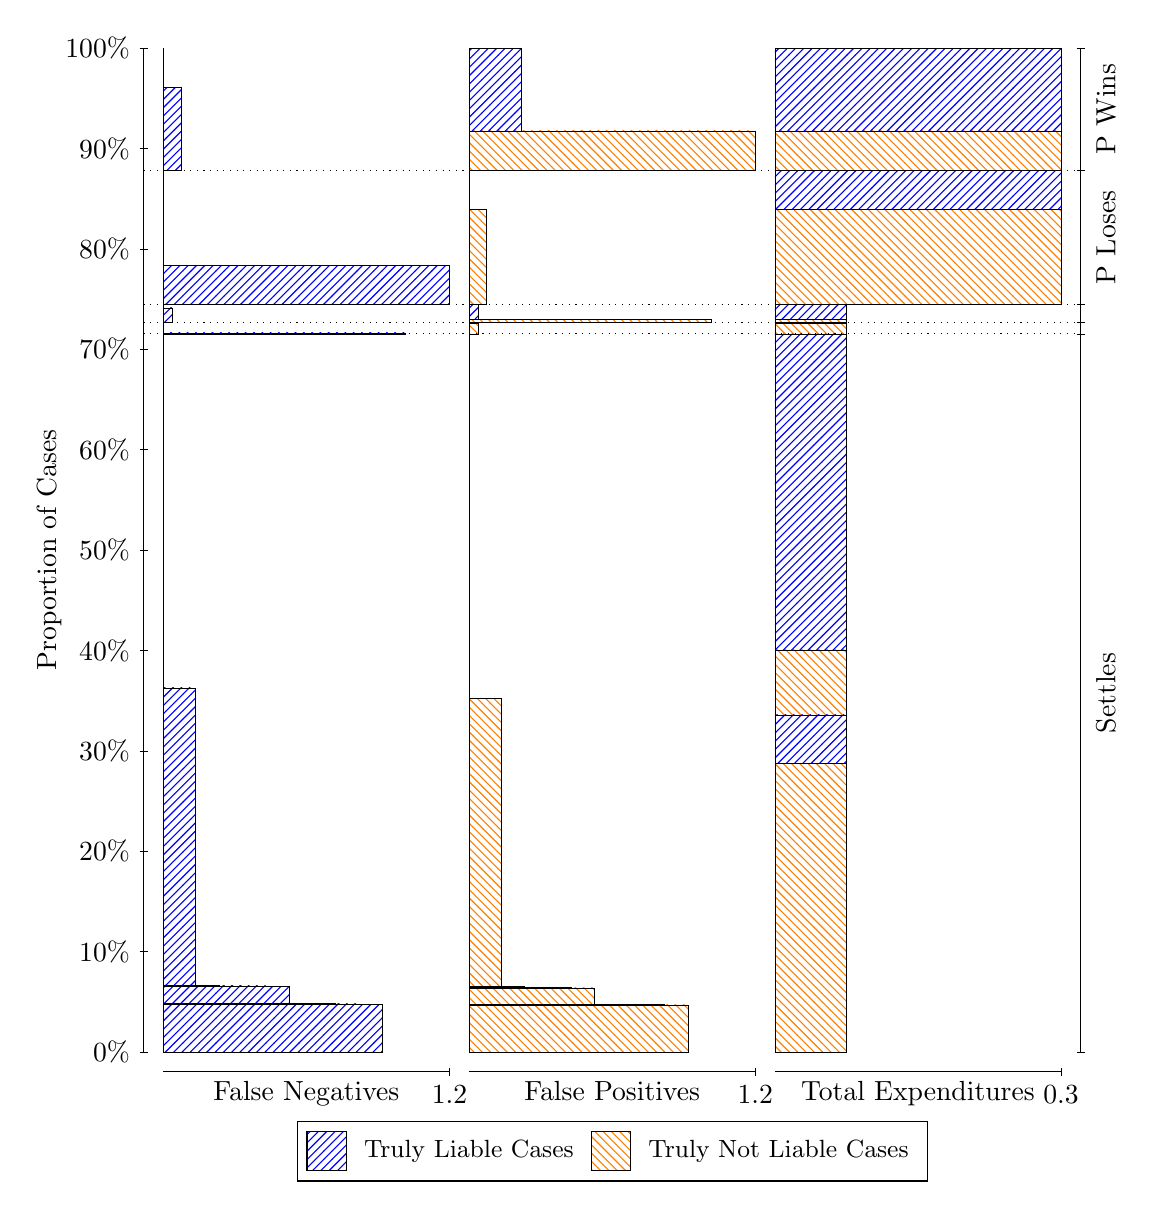
\begin{tikzpicture}
\draw[black, very thin] (1.5,1.75) -- (1.5,14.5);
\node[rotate=90, anchor=center] at (0.3, 8.125) {Proportion of Cases};
\draw[black, very thin] (1.45,1.75) -- (1.55,1.75);
\node[anchor=east] at (1.45, 1.75) {0\%};
\draw[black, very thin] (1.45,3.025) -- (1.55,3.025);
\node[anchor=east] at (1.45, 3.025) {10\%};
\draw[black, very thin] (1.45,4.3) -- (1.55,4.3);
\node[anchor=east] at (1.45, 4.3) {20\%};
\draw[black, very thin] (1.45,5.575) -- (1.55,5.575);
\node[anchor=east] at (1.45, 5.575) {30\%};
\draw[black, very thin] (1.45,6.85) -- (1.55,6.85);
\node[anchor=east] at (1.45, 6.85) {40\%};
\draw[black, very thin] (1.45,8.125) -- (1.55,8.125);
\node[anchor=east] at (1.45, 8.125) {50\%};
\draw[black, very thin] (1.45,9.4) -- (1.55,9.4);
\node[anchor=east] at (1.45, 9.4) {60\%};
\draw[black, very thin] (1.45,10.675) -- (1.55,10.675);
\node[anchor=east] at (1.45, 10.675) {70\%};
\draw[black, very thin] (1.45,11.95) -- (1.55,11.95);
\node[anchor=east] at (1.45, 11.95) {80\%};
\draw[black, very thin] (1.45,13.225) -- (1.55,13.225);
\node[anchor=east] at (1.45, 13.225) {90\%};
\draw[black, very thin] (1.45,14.5) -- (1.55,14.5);
\node[anchor=east] at (1.45, 14.5) {100\%};

\draw[black, very thin] (13.4,1.75) -- (13.4,14.5);
\draw[black, very thin] (13.35,1.75) -- (13.45,1.75);
\node[anchor=west] at (13.35, 1.75) {};
\draw[black, very thin] (13.35,10.869) -- (13.45,10.869);
\node[anchor=west] at (13.35, 10.869) {};
\draw[black, very thin] (13.35,11.015) -- (13.45,11.015);
\node[anchor=west] at (13.35, 11.015) {};
\draw[black, very thin] (13.35,11.241) -- (13.45,11.241);
\node[anchor=west] at (13.35, 11.241) {};
\draw[black, very thin] (13.35,12.949) -- (13.45,12.949);
\node[anchor=west] at (13.35, 12.949) {};
\draw[black, very thin] (13.35,14.5) -- (13.45,14.5);
\node[anchor=west] at (13.35, 14.5) {};

\draw[black, very thin, pattern color=blue, pattern=north east lines] (1.75,1.75) rectangle (4.5306,2.3575);
\draw[black, very thin, pattern color=blue, pattern=north east lines] (1.75,2.3575) rectangle (4.234,2.3613);
\draw[black, very thin, pattern color=blue, pattern=north east lines] (1.75,2.3613) rectangle (3.9374,2.3653);
\draw[black, very thin, pattern color=blue, pattern=north east lines] (1.75,2.3653) rectangle (3.6408,2.3692);
\draw[black, very thin, pattern color=blue, pattern=north east lines] (1.75,2.3692) rectangle (3.3442,2.5873);
\draw[black, very thin, pattern color=blue, pattern=north east lines] (1.75,2.5873) rectangle (3.0476,2.5886);
\draw[black, very thin, pattern color=blue, pattern=north east lines] (1.75,2.5886) rectangle (2.751,2.5899);
\draw[black, very thin, pattern color=blue, pattern=north east lines] (1.75,2.5899) rectangle (2.4544,2.5912);
\draw[black, very thin, pattern color=blue, pattern=north east lines] (1.75,2.5912) rectangle (2.1578,6.3747);
\draw[black, very thin, pattern color=orange, pattern=north west lines] (1.75,6.3747) rectangle (1.75,10.869);
\draw[black, very thin, pattern color=blue, pattern=north east lines] (1.75,10.869) rectangle (4.8272,10.882);
\draw[black, very thin, pattern color=orange, pattern=north west lines] (1.75,10.882) rectangle (1.75,11.015);
\draw[black, very thin, pattern color=blue, pattern=north east lines] (1.75,11.015) rectangle (1.8612,11.2);
\draw[black, very thin, pattern color=orange, pattern=north west lines] (1.75,11.2) rectangle (1.75,11.241);
\draw[black, very thin, pattern color=blue, pattern=north east lines] (1.75,11.241) rectangle (5.3833,11.741);
\draw[black, very thin, pattern color=orange, pattern=north west lines] (1.75,11.741) rectangle (1.75,12.949);
\draw[black, very thin, pattern color=blue, pattern=north east lines] (1.75,12.949) rectangle (1.9724,14.001);
\draw[black, very thin, pattern color=orange, pattern=north west lines] (1.75,14.001) rectangle (1.75,14.5);
\draw[black, very thin, pattern color=orange, pattern=north west lines] (5.6333,1.75) rectangle (8.4139,2.3471);
\draw[black, very thin, pattern color=orange, pattern=north west lines] (5.6333,2.3471) rectangle (8.1173,2.3496);
\draw[black, very thin, pattern color=orange, pattern=north west lines] (5.6333,2.3496) rectangle (7.8207,2.3521);
\draw[black, very thin, pattern color=orange, pattern=north west lines] (5.6333,2.3521) rectangle (7.5241,2.3546);
\draw[black, very thin, pattern color=orange, pattern=north west lines] (5.6333,2.3546) rectangle (7.2276,2.5646);
\draw[black, very thin, pattern color=orange, pattern=north west lines] (5.6333,2.5646) rectangle (6.931,2.5646);
\draw[black, very thin, pattern color=orange, pattern=north west lines] (5.6333,2.5646) rectangle (6.931,2.5693);
\draw[black, very thin, pattern color=orange, pattern=north west lines] (5.6333,2.5693) rectangle (6.6344,2.574);
\draw[black, very thin, pattern color=orange, pattern=north west lines] (5.6333,2.574) rectangle (6.3378,2.5786);
\draw[black, very thin, pattern color=orange, pattern=north west lines] (5.6333,2.5786) rectangle (6.0412,6.2438);
\draw[black, very thin, pattern color=blue, pattern=north east lines] (5.6333,6.2438) rectangle (5.6333,10.869);
\draw[black, very thin, pattern color=orange, pattern=north west lines] (5.6333,10.869) rectangle (5.7446,11.001);
\draw[black, very thin, pattern color=blue, pattern=north east lines] (5.6333,11.001) rectangle (5.6333,11.015);
\draw[black, very thin, pattern color=orange, pattern=north west lines] (5.6333,11.015) rectangle (8.7105,11.056);
\draw[black, very thin, pattern color=blue, pattern=north east lines] (5.6333,11.056) rectangle (5.7446,11.241);
\draw[black, very thin, pattern color=orange, pattern=north west lines] (5.6333,11.241) rectangle (5.8558,12.449);
\draw[black, very thin, pattern color=blue, pattern=north east lines] (5.6333,12.449) rectangle (5.6333,12.949);
\draw[black, very thin, pattern color=orange, pattern=north west lines] (5.6333,12.949) rectangle (9.2667,13.448);
\draw[black, very thin, pattern color=blue, pattern=north east lines] (5.6333,13.448) rectangle (6.3007,14.5);
\draw[black, very thin, pattern color=orange, pattern=north west lines] (9.5167,1.75) rectangle (10.425,5.4198);
\draw[black, very thin, pattern color=blue, pattern=north east lines] (9.5167,5.4198) rectangle (10.425,6.0312);
\draw[black, very thin, pattern color=orange, pattern=north west lines] (9.5167,6.0312) rectangle (10.425,6.8551);
\draw[black, very thin, pattern color=blue, pattern=north east lines] (9.5167,6.8551) rectangle (10.425,10.869);
\draw[black, very thin, pattern color=orange, pattern=north west lines] (9.5167,10.869) rectangle (10.425,11.001);
\draw[black, very thin, pattern color=blue, pattern=north east lines] (9.5167,11.001) rectangle (10.425,11.015);
\draw[black, very thin, pattern color=orange, pattern=north west lines] (9.5167,11.015) rectangle (10.425,11.056);
\draw[black, very thin, pattern color=blue, pattern=north east lines] (9.5167,11.056) rectangle (10.425,11.241);
\draw[black, very thin, pattern color=orange, pattern=north west lines] (9.5167,11.241) rectangle (13.15,12.449);
\draw[black, very thin, pattern color=blue, pattern=north east lines] (9.5167,12.449) rectangle (13.15,12.949);
\draw[black, very thin, pattern color=orange, pattern=north west lines] (9.5167,12.949) rectangle (13.15,13.448);
\draw[black, very thin, pattern color=blue, pattern=north east lines] (9.5167,13.448) rectangle (13.15,14.5);
\draw[black, dotted] (1.5,10.869) -- (13.4,10.869);
\draw[black, dotted] (1.5,11.015) -- (13.4,11.015);
\draw[black, dotted] (1.5,11.241) -- (13.4,11.241);
\draw[black, dotted] (1.5,12.949) -- (13.4,12.949);
\draw[black, very thin] (1.75,1.5) -- (5.3833,1.5);
\node[anchor=north] at (3.5667, 1.5) {False Negatives};
\draw[black, very thin] (5.3833,1.45) -- (5.3833,1.55);
\node[anchor=north] at (5.3833, 1.45) {1.2};

\draw[black, very thin] (5.6333,1.5) -- (9.2667,1.5);
\node[anchor=north] at (7.45, 1.5) {False Positives};
\draw[black, very thin] (9.2667,1.45) -- (9.2667,1.55);
\node[anchor=north] at (9.2667, 1.45) {1.2};

\draw[black, very thin] (9.5167,1.5) -- (13.15,1.5);
\node[anchor=north] at (11.333, 1.5) {Total Expenditures};
\draw[black, very thin] (13.15,1.45) -- (13.15,1.55);
\node[anchor=north] at (13.15, 1.45) {0.3};

\node[black, centered, rotate=90] at (13.72, 6.3093) {Settles};


\node[black, centered, rotate=90] at (13.72, 12.095) {P Loses};
\node[black, centered, rotate=90] at (13.72, 13.725) {P Wins};

\draw (7.449999999999999,1.5) node[draw=none] (baseCoordinate) {};
\begin{scope}[align=center]
        \matrix[scale=0.5, draw=black, below=0.5cm of baseCoordinate, nodes={draw}, column sep=0.1cm]{
            \node[rectangle, draw, minimum width=0.5cm, minimum height=0.5cm, pattern=north east lines, pattern color=blue] {}; &
            \node[draw=none, font=\small] (B) {Truly Liable Cases}; &
            \node[rectangle, draw, minimum width=0.5cm, minimum height=0.5cm, pattern=north west lines, pattern color=orange] {}; &
            \node[draw=none, font=\small] (B) {Truly Not Liable Cases}; \\
            };
\end{scope}

\end{tikzpicture}
\end{document}